\documentclass[12pt,a4paper]{article}
\usepackage[utf8]{inputenc}
\usepackage[german]{babel}
\usepackage[T1]{fontenc}
\usepackage{amsmath}
\usepackage{amsfonts}
\usepackage{amssymb}
\usepackage{graphicx}
\usepackage{siunitx}
\usepackage[left=2cm,right=2cm,top=2cm,bottom=2cm]{geometry}
\author{Tim}

\begin{document}
	\setlength{\parindent}{0pt} 
	\begin{center}
		{\LARGE Versuchsprotokoll}\\
		\begin{large}
			zum Grundpraktikum Physik Teil II\\[0.4cm]
			an der RWTH Aachen\\
			I. Physikalisches Institut B\\[4.5cm]
			\Large\textbf{\textsl{Optik I}}\\[4cm]
			\normalsize\textit{vorgelegt\\von}\\[0.4cm]
			\large{Moritz Berger\\Tim Herbermann\\Gerald Kolter\\Sebastian Siebert}\\[1cm]
			\large \textit{Gruppe A07} \\ [3cm]
			\large \textbf{Sommersemester 2017}
		\end{large}
	\end{center}
	\newpage
	
	\tableofcontents
	\newpage
	
	\section{Prismenspektrometer}
	
	\subsection{Grundlagen}
	Grundlage des Versuches ist die spektrale Zerlegung des Lichts mittels eines Prismas. Ursächlich dafür ist das Zusammenspiel von Lichtbrechung und Dispersion des Lichts beim Durchlaufen von Materie, da der Brechungsindex von der Wellenlänge der durchlaufenden elektromagnetischen Strahlung abhängt.
	
	Das Brechungsgesetz an der Grenzfläche von zwei Medien mit unterschiedlichem Brechungsindex $n_1$ und $n_2$ lautet:
	
	\begin{equation}
	n_1 sin(\alpha_1) = n_2 sin(\alpha_2)
	\end{equation}
	
	Mit diesem und unter Ausnutzung geometrischer Beziehungen in einem Dreieck kann ein Zusammenhang zwischen Brechungsindex des Prismas bei einer gegeben Wellenlänge und Minimalablenkung hergeleitet werden.
	
	\begin{equation}
	n = \frac{sin(\frac{\delta_{min}+\epsilon}{2})}{sin(\frac{\epsilon}{2})}
	\end{equation}
	
	Das Auflösungsvermögen ist definiert durch
	
	\begin{equation}
	A = \frac{\lambda}{\Delta \lambda}
	\end{equation} 
	
	und ist ein Maß dafür, ob zwei Spektrallinien mit Wellenlängen $\lambda$ und $\lambda + \Delta \lambda$ getrennt werden können.
	
	An einem Prisma ergibt sich für das Auflösungsvermögen der Zusammenhang
	
\begin{equation}
A = \dfrac{dn}{d\lambda}\cdot 2\cdot a\cdot\dfrac{sin\left(\dfrac{\epsilon}{2}\right)}{cos\left(\dfrac{\delta_{min}+\epsilon}{2}\right)}
\label{eq:Auflosung}
\end{equation}
	
	wobei $\frac{dn}{d\lambda}$ die Dispersion des Prismas und a die Breite der beleuchteten Fläche auf dem Prisma ist.

\begin{figure}
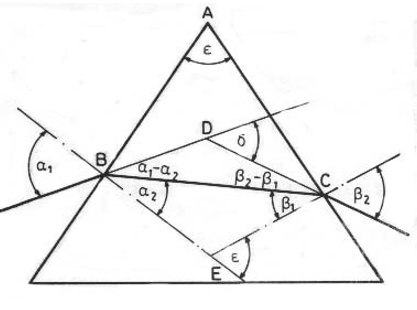
\includegraphics[scale=1.0]{Bilder/prisma}
\caption{Strahlengang im Prisma}
\label{fig:Prisma}
\end{figure}

	
	
	\subsection{Aufbau und Durchführung}
	Durch eine Kollimatorlinse werden aus dem Licht der Spektrallampe ebene Wellenfronten erzeugt. Diese werden mit dem einem Drehteller befindlichen Prisma gebrochen. Das gebrochene Spaltbild wird mit einem schwenkbaren Fernrohr beobachtet. Die relative Position des Fernrohrs kann dabei auf 1' genau abgelesen werden.
	Der Aufbau ist in Abbildung \ref{fig:AufbauPrisma} gezeigt.
	
	\begin{figure}
		\begin{center}
			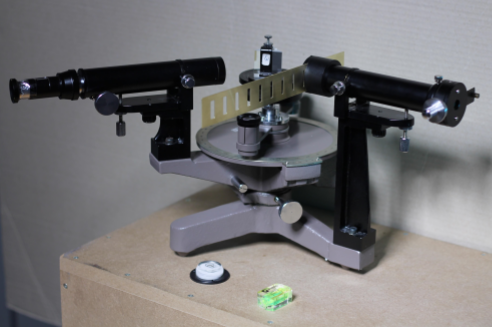
\includegraphics[scale=1.0]{Bilder/AufbauPrisma}
			\caption{Aufbau des Versuches. Auf dem Kollimatorrohr befindet sich eine Schlitzblende, welche nur im Versuch zum Auflösungsvermögen verwendet wurde. Das Bild wurde dem Praktikumsskript entnommen (S.21)}
			\label{fig:AufbauPrisma}
		\end{center}
	\end{figure}
	
	In den ersten beiden Teilversuchen werden zunächst die Minimalablenkungen des Prismas für bestimmte Spektrallinien bestimmt.
	Durch gleichsinniges Drehen von Prismenteller und Fernrohr wandern auch die Spektrallinien, zunächst in die eine und dann in die andere Richtung. Der Umkehrpunkt entspricht dabei der Minimalablenkung. Die entsprechende Spektrallinie wird mit dem Fernrohr anvisiert und die relative Position notiert. Man wiederholt die Messung, diesmal trifft das Licht allerdings auf der anderen Prismenseite auf. Dann gilt für die Minimalablenkung
	
	\begin{equation}
	2 \delta_{min} = \psi_2-\psi_1
	\end{equation}
	
	wobei $\psi_i$ die relativen Positionen der Umkehrpunkte sind.
	Zur Bestimmung der statistischen Unsicherheit auf die $\psi_i$ wurde eine Rauschmessung an der $\psi_1$-Position der blau-grünen Cadmiumlinie ($\lambda=508,58nm$) durchgeführt.
	
	Für die übrigen Positionen der Spektrallinien wurde die Messung drei (bzw. fünf) mal wiederholt. Der Fehler auf die sich so ergebenden Mittelwert ist dann $\sigma_{\psi}=\frac{\sigma_{psi}}{\sqrt{N}}$.
	
	Es ergeben sich damit die Minimalablenkungen und der Fehler auf selbige für jede vermessene Spektrallinie.
	
	\begin{equation}
	\sigma_{\delta} = \frac{\sqrt{\sigma_{\psi_1}^2+\sigma_{\psi_2}^2}}{2}
	\end{equation}
	
	Damit folgt für die Brechungsindizes bei den entsprechenden Wellenlängen der Zusammenhang (vgl. Grundlagen):
	
	\begin{equation}
	n = \frac{sin(\frac{\delta_{min}+\epsilon}{2})}{sin(\frac{\epsilon}{2})}
	\end{equation}
	
	Die Unsicherheit ergibt sich mittels Gaußscher Fehlerfortpflanzung:
	
	\begin{equation}
	\sigma_n = \frac{cos(\frac{\delta_{min}+\epsilon}{2})}{sin(\frac{\epsilon}{2})} \frac{\sigma_{\delta_{min}}}{2}
	\end{equation}

Nachdem man die Dispersionskurve ermittelt hat, wird die Spektrallampe ausgetauscht und das SPektrum der neuen Lampe bestimmt. 
Dabei ermittelt man zuerst mit dem gleichen Verfahren die Brechungsindizes der Spektrallinien und ordnet diesen dann über die Dispersionskurve eine Wellenlänge zu.
	
Zur Abschätzung des Auflösungsvermögens wird eine Schlitzblende auf das Kollimatorrohr gesteckt. Mit dem Fernrohr wird die gelbe Doppellinie des Quecksilberspektrums anvisiert.  Anschließend wird die beleuchtete Fläche des Prismas durch Vorschalten immer kleinerer Blenden soweit verkleinert, dass die Doppellinie gerade noch getrennt werden kann. Daraus wird eine Abschätzung des Auflösungsvermögens bestimmt (vgl. Grundlagen). 
	
	
	\subsection{Auswertung}
	
	\subsubsection{Rauschmessung}
	
	Das Ergebnis der Rauschmessung zur Bestimmung des statistischen Fehlers für die Winkelmessung findet sich in Tabelle \ref{tab:RauschenPrisma}.
	
	\begin{figure}
		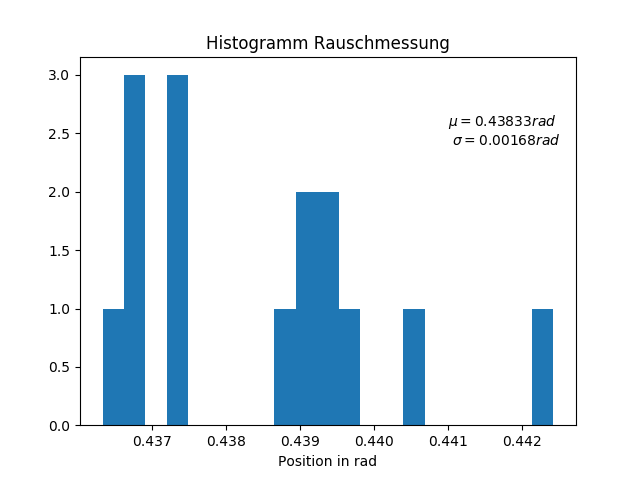
\includegraphics[scale=1.0]{Bilder/HistRauschen.png}
		\caption{Grafische Darstellung der Rauschmessung mit empirischem Mittelwert und empirischer Standardabweichung. Die Bin-Breite entspricht der Ablesegenauigkeit von einer Bogenminute. Die Messung wurde 15 mal durchgeführt.}
		\label{fig:HistRauschen}
	\end{figure}
	
	Die Rauschmessung ergibt eine statistische Unsicherheit auf die $\psi_i$ von $\sigma_{\psi_i} = 0.0017 rad$ bzw. $\sigma_{\psi_i} = 5.8'$ (vgl. Abb \ref{fig:HistRauschen}.)
	
	\begin{table}
		\begin{center}
			\begin{tabular}{|c|c|}
				\hline 
				$\psi_1$ & $\psi_2$ \\ 
				\hline 
				25$^{\circ}$3' & 147$^{\circ}$21' \\ 
				\hline 
				25$^{\circ}$1' & 147$^{\circ}$22' \\ 
				\hline 
				25$^{\circ}$0'& 147$^{\circ}$13' \\ 
				\hline 
				25$^{\circ}$1' & 147$^{\circ}$11' \\ 
				\hline 
				25$^{\circ}$1' & 147$^{\circ}$16' \\ 
				\hline 
				25$^{\circ}$3' & \\ 
				\hline 
				25$^{\circ}$9' & \\ 
				\hline 
				25$^{\circ}$3' & \\ 
				\hline 
				25$^{\circ}$10' & \\ 
				\hline 
				25$^{\circ}$20' & \\ 
				\hline 
				25$^{\circ}$14' & \\ 
				\hline 
				25$^{\circ}$11' & \\ 
				\hline 
				25$^{\circ}$9' & \\ 
				\hline 
				25$^{\circ}$8' & \\ 
				\hline 
				25$^{\circ}$10' & \\ 
				\hline 
				
			\end{tabular} 
			
			\caption{Rohdaten der grün-blauen Cadmiumlinie. Die Messwerte auf $\psi_1$ dienen als Rauschmessung für die statistische Unsicherheit .}
			\label{tab:RauschenPrisma}
		\end{center}
	\end{table}
	
	
	\subsubsection{Dispersionskurve}
	In diesem Teilversuch wurde die Dispersionskurve des verwendeten Prismas mithilfe einer Quecksilber-Cadmium-Lampe vermessen.
	
	
	\paragraph{Rohdaten}
	
	\begin{table}
		\begin{center}
			\begin{tabular}{|c|c|}
				\hline
				$\psi_1$ & $\psi_2$ \\
				\hline
				$\lambda =$404.66nm & \\
				\hline
				21$^{\circ}$2' &151$^{\circ}$15' \\
				\hline
				21$^{\circ}$0' &151$^{\circ}$14' \\
				\hline
				20$^{\circ}$56' &151$^{\circ}$18' \\ 
				\hline
				$\lambda =$435.83nm & \\
				\hline
				22$^{\circ}$43' &149$^{\circ}$34' \\
				\hline
				22$^{\circ}$45' &149$^{\circ}$33' \\ 
				\hline
				22$^{\circ}$42' &149$^{\circ}$33' \\ 
				\hline
				$\lambda =$467.81nm & \\
				\hline
				23$^{\circ}$55' &148$^{\circ}$22' \\
				\hline
				23$^{\circ}$54' &148$^{\circ}$24' \\
				\hline
				23$^{\circ}$57' &148$^{\circ}$20' \\ 
				\hline
				$\lambda =$479.99nm & \\
				\hline
				24$^{\circ}$22' &147$^{\circ}$56' \\ 
				\hline
				24$^{\circ}$24' &148$^{\circ}$0' \\ 
				\hline
				24$^{\circ}$18' &148$^{\circ}$2' \\ 
				\hline
				$\lambda =$564.07nm & \\
				\hline
				25$^{\circ}$53' &146$^{\circ}$24' \\
				\hline
				25$^{\circ}$54' &146$^{\circ}$25' \\
				\hline
				25$^{\circ}$54' &146$^{\circ}$22' \\ 
				\hline
				$\lambda =$579.07nm & \\
				\hline
				26$^{\circ}$34' &145$^{\circ}$48' \\
				\hline
				26$^{\circ}$32' &145$^{\circ}$44' \\
				\hline
				26$^{\circ}$33' &145$^{\circ}$44' \\ 
				\hline
				$\lambda =$643.85nm & \\
				\hline
				27$^{\circ}$20' &144$^{\circ}$57' \\
				\hline
				27$^{\circ}$20' &144$^{\circ}$55' \\
				\hline
				27$^{\circ}$24' &144$^{\circ}$59' \\
				\hline
			\end{tabular}
			\caption{Rohdaten für die Position der beiden Umkehrpunke für die vermessenen Spektrallinien der HgCa-Lampe. Die Wellenlängen sind dem Praktikumsskript (S.19) entnommen worden.}
			\label{tab:RohdatenDispersion}
		\end{center}
	\end{table}
	
	
	Die Rohdaten der restlichen Spektrallinien, welche Vermessen wurden sind nach Wellenlänge sortiert in Tabelle \ref{tab:RohdatenDispersion} dargestellt.
	
	
	\paragraph{Auswertung}
	
	\begin{table}
		\begin{center}
			\begin{tabular}{|c|c|c|}
				\hline
				435.83 & 1.1068 $\pm$ 0.0007 & 1.7611 $\pm$ 0.0003 \\ 
				\hline
				467.81 & 1.086 $\pm$ 0.0007 & 1.7511 $\pm$ 0.0003 \\
				\hline
				479.99 & 1.0789 $\pm$ 0.0007 & 1.7477 $\pm$ 0.0003 \\
				\hline
				508.58 & 1.0661 $\pm$ 0.0004 & 1.7414 $\pm$ 0.0002 \\
				\hline
				546.07 & 1.0516 $\pm$ 0.0007 & 1.7342 $\pm$ 0.0003 \\
				\hline
				579.07 & 1.0403 $\pm$ 0.0007 & 1.7286 $\pm$ 0.0003 \\
				\hline
				643.85 & 1.0262 $\pm$ 0.0007 & 1.7215 $\pm$ 0.0003 \\ 
				\hline
			\end{tabular}
			\caption{Ergebnisse der Auswertung. Dargestellt ist der bestimmte minimale Ablenkungswinkel mit Unsicherheit für jede vermessene Linie sowie die sich daraus ergebenden Brechungsindizes.}
			\label{tab:AuswertungDispersion}
		\end{center}
	\end{table}
	
	\begin{figure}
		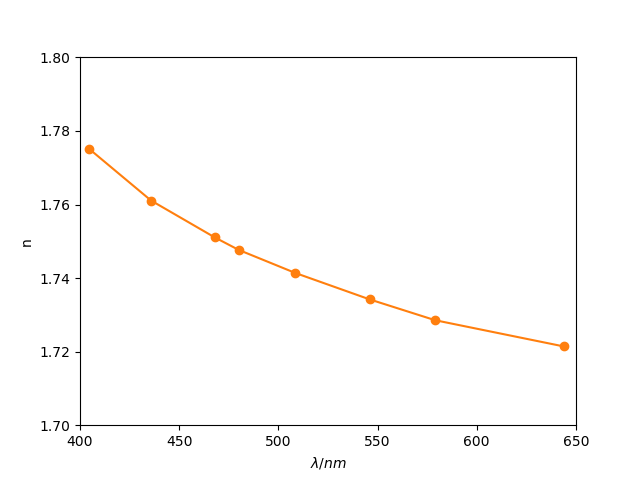
\includegraphics[scale=1.0]{Bilder/Dispersionskurve.png}
		\caption{Die Dispersionskurve des verwendeten Prismas. Die Fehlerbalken auf die n-Werte sind relativ klein und somit nicht erkennbar. Die einzelnen Messpunkte wurden zur Veranschaulichung verbunden.}\label{fig:Dispersionskurve}
	\end{figure}
	
	\begin{figure}
		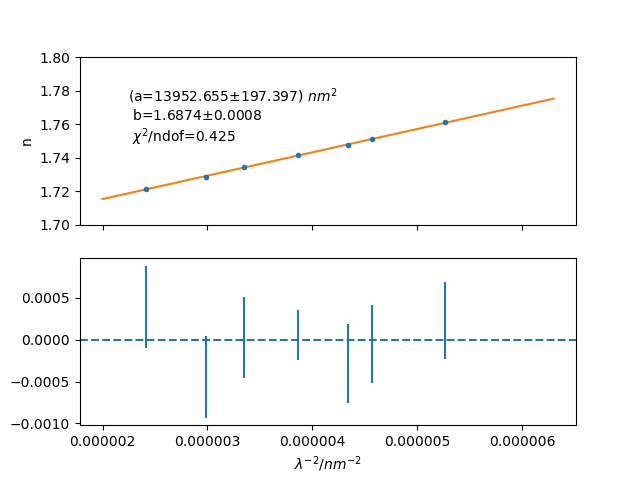
\includegraphics[scale=1.0]{Bilder/Regression.png}
		\caption{Auftragung von n gegen $1/\lambda^2$. Das beste Anpassung ergab sich für eine Anpassungsgerade der Form $n(\lambda) = \frac{a}{\lambda^2} + b $} und unter Vernachlässigung der violetten Linie bei ca 404nm. Auch hier sind die Fehlerbalken aufgrund der geringen Größe kaum erkennbar.
		\label{fig:RegressionDispersion}
	\end{figure}
	
	
	Wie in der Durchführung beschrieben kann nun aus den Daten die Minimalablenkung $\delta_{min}$ und der entsprechende Fehler, sowie aus diesen der Brechungsindex und seine Unsicherheit für die jeweiligen Wellenlängen berechnet werden.
	Die Werte sind in Tabelle \ref{tab:AuswertungDispersion} dargestellt.
	
	Durch Auftragen des Brechungsindex gegen die Wellenlänge erhält man die Dispersionskurve (Abb. \ref{fig:Dispersionskurve}).
	
An dieser Kurve wird nun eine Lineare Regression der Form
\begin{equation}
n(\lambda) = \dfrac{a}{\lambda^2} + b
\label{eq:linreg_Prisma}
\end{equation} durchgeführt. Diese ist in Abblidung
\ref{fig:RegressionDispersion} dargestellt. Die Vernachlässigung der violetten Linie bei etwa 404nm wird damit begründet, dass diese Linie schwer zu vermessen war und stark vom näherungsweise linearen Zusammenhang der anderen Datenpunkte abweicht.

\paragraph{Fazit}
Die Bestimmung der Brechungsindizes ist mit einer relativen Unsicherheit im Subpromillbereich gelungen. Der sehr gute $\chi^2/ndof$ Wert in der Anpassung unterstreicht die Übereinstimmung mit dem theoretischen Modell.

\subsubsection{Spektrallinien}
Im folgenden Versuchsteil soll mithilfe der nun bestimmten Dispersionskurve das Spektrum einer unbekannten Spektrallampe ermittelt werden.
\begin{table}
\begin{tabular}{|c|c|c||c|c|c|}
\hline 
 & $\psi_1$ & $\psi_2$ & & $\psi_1$ & $\psi_2$ \\ 
\hline 
Linie 1(rot) & $27^\circ 20'$ & $145^\circ 02'$ & Linie 3(blau) & $24^\circ 06'$ & $148^\circ 11'$\\ 
\hline 
 & $27^\circ 16'$ & $145^\circ 03'$& & $24^\circ 07'$ & $148^\circ 10'$\\
\hline
\hline 
\hline 
Linie 2(blau) & $24^\circ 22'$ & $147^\circ 53'$ & Linie 4(blau) & $23^\circ 59'$ & $148^\circ 20'$\\ 
\hline 
 & $24^\circ 21'$ & $147^\circ 24'$&  & $23^\circ 57'$ & $148^\circ 22'$\\ 
\hline 
\end{tabular} 
\caption{Rohdaten der Spektrallinien beim Prisma}
\label{tab:Spektrallinien_rohdaten}
\end{table}

\paragraph{Bestimmung des Brechungsindex}
Die Bestimmung der Brechungsindizes verläuft analog zum vorherigen Teilversuch. Die ermittelten Winkel sind in Tabelle \ref{tab:Spektrallinien_rohdaten} aufgelistet.
Der Fehler auf diesen Werten folgt weiterhin aus der Rauschmessung und beträgt
\begin{equation}
\sigma_{\psi} = 0.0017 rad
\end{equation}\\
und der Fehler auf $\delta_{min}$
\begin{equation}
\sigma_{\delta} = 0.0008 rad
\end{equation}\\
Die errechneten Ergebnisse für $\delta_{min}$ und den Brechungsindex n sind in Tabelle \ref{tab:Spekrallinien_Brechungsndex} aufgelistet.

\begin{table}
\begin{tabular}{|c|c|c|c|c|}
\hline
 & Linie 1 & Linie 2 & Linie 3 & Linie 4\\
\hline
$\delta_{min}$ & $58.8708^\circ$ & $61.6417^\circ$ & $62.0333^\circ$ & $62.1917^\circ$\\
\hline
$n$ & $1.72211\pm 0.0006$ & $1.74619\pm 0.0006$ & $1.74952\pm 0.0006$ & $1.75086\pm 0.0006$\\
\hline
\end{tabular}
\caption{Mithilfe des oben beschriebenen Verfahrens ermittelte Werte für minimaler Brechungswinkel und Brechzahl}
\label{tab:Spekrallinien_Brechungsndex}
\end{table}
\paragraph{Ermittlung der Wellenlängen}
Mithilfe der vorher bestimmten Dispersionskurve wird nun jeder Brechzahl die dazugehörige Wellenlänge zugeordnet. Dabei wird die Gleichung \ref{eq:linreg_Prisma} folgendermaßen umgestellt:
\begin{equation}
\lambda = \sqrt{\dfrac{a}{n-b}}
\end{equation}
Die Fehlerfortpflanzung auf dieser Formel sieht folgendermaßen aus:
\begin{equation}
\sigma_{\lambda} = \sqrt{\left(\dfrac{\sqrt{\dfrac{a}{n-b}}}{2\cdot a}\cdot \sigma_{a}\right)^2 + \left(\dfrac{a}{2\cdot (n-b)^2\cdot \sqrt{\dfrac{a}{n-b}}}\right)^2\cdot (\sigma_n^2 + \sigma_b^2)}
\end{equation}
Die sich daraus ergebenen Endwerte sind in Tabelle \ref{tab:Spektrallinien_Endergebnis} aufgelistet und wurden in Abbildung \ref{fig:Spektrum_Zink} nochmal visualisiert.
\begin{table}
\begin{tabular}{|c|c|c|c|c|}
\hline
 & Linie 1 & Linie 2 & Linie 3 & Linie 4\\
\hline
$\lambda [nm]$ & $634.08\pm 5.02 $ & $487.17\pm 3.74$ & $473.96\pm 3.53$ & $468.94\pm 4.45$\\
\hline
Literaturwerte[nm] & 636.23 & 481.05 & 472.22 & 468.01\\
\hline
Standardabw.& 0.43 & 1.63 & 0.49 & 0.21\\
\hline
\end{tabular}
\caption{Ergebnisse der Wellenlängenbestimmung und Vergleich mit den Literaturwerten. Es wurde außerdem die Anzahl der Standardabweichungen zwischen den Werten angegeben.}
\label{tab:Spektrallinien_Endergebnis}
\end{table}
\paragraph{Fazit}
Die ermittelten Wellenlängen der Spektrallinien haben eine Ungenauigkeit von c.a 1\% und liegen zum größten Teil innerhalb einer Standardabweichung vom Literaturwert entfernt. Es handelt sich also bei der Lampe tatsächlich um eine Zink-Lampe. Die Bestimmung ist also geglückt.
\begin{figure}
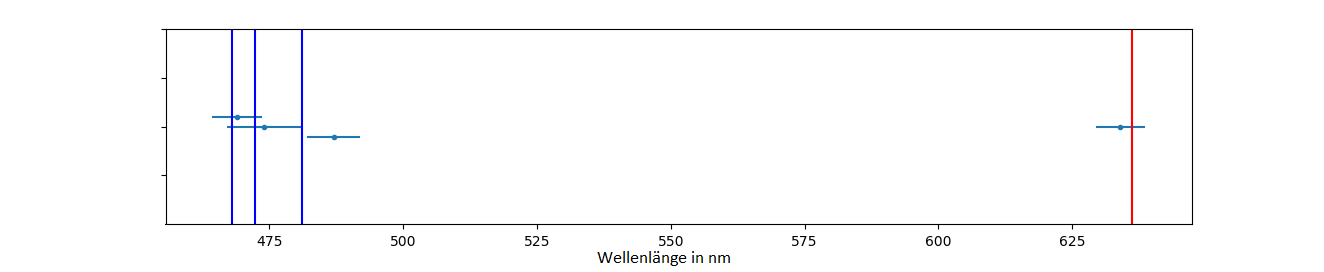
\includegraphics[scale=0.85]{Bilder/Spektrum_Zink.png}
\caption{Visualisierung der Messergebnisse und des erwarteten Spektrums mit den Wellenlängen $\lambda = 468nm, 472nm, 481nm, 636nm$. Die senkrechten Linien entsprechen den Literaturwerten und die Punkte mitsamt ihren Ungenauigkeiten den Messergebnissen.}
\label{fig:Spektrum_Zink}
\end{figure}
\subsubsection{Auflösungsvermögen}
\paragraph{Auswertung}
Das Auflösungsvermögen wird mithilfe von Formel \ref{eq:Auflosung} bestimmt.
Die Steigung ergibt sich dabei durch Ableiten der Dispersionskurve an der Stelle $\lambda = 579.07 nm$. Das zu dieser Wellenlänge gehörige $\delta_{min}$ wurde ebenfalls bereits in 1.Teilversuch bestimmt und kann in Tabelle \ref{tab:AuswertungDispersion} abgelesen werden. \\
Der Faktor a beschreibt die Breite des Spaltes. Diese wurde im Versuch von 6 mm an immer um 0.5 mm verkleinert, bis die Aufspaltung der Linien nicht mehr sichtbar war. Die Ergebnisse sind in Tabelle \ref{tab:Auflosung_Prisma} angegeben.
\begin{table}
\begin{tabular}{|c|c|c|c|c|c|c|}
\hline
a[mm] & 6 & 5.5 & ... & 1.5 & 1 & 0.5\\
\hline
Trennbar? & ja & ja & ja & ja & gerade so & nein\\
\hline
\end{tabular}
\caption{Überprüfung der Auflösbarkeit der beiden gelben Spektrallinien ($\lambda = 579.07nm$ und $\lambda = 576.96nm$). Ab einer Spaltbreite von 0.5 mm konnte man die Linien nicht mehr unterscheiden.}
\label{tab:Auflosung_Prisma}
\end{table}

	Wegen der sehr großen Abständen zwischen den Spaltbreiten macht eine Fehlerbetrachtung keinen Sinn.\\
	Für die experimentell bestimmte Auflösung folgt:
	\begin{equation}
	A \approx 286
	\end{equation}
	Der theoretisch erwartete Wert beträgt:
	\begin{equation}
	A = \dfrac{\lambda}{\Delta \lambda} = \dfrac{579.1 nm}{2.1 nm} = 276
	\end{equation}
	Wegen der hohen Ungenauigkeit kann man annehmen, dass der ermittelte Wert mit der theoretischen Erwartung übereinstimmt.
	
	
\subsection{Fazit}
Der prinzipielle Verlauf der Dispersionskurve entspricht der Erwartung im sichtbaren Bereich. Auch die lineare Anpassung an die Sellmeier-Formel ist mit einem $\chi^2/ndof$ von 0,86 gut gelungen.\\
Die Bestimmung des Spektrums der Zinklampe ergab die Wellenlängen $634nm, 487nm, 473 nm, 469nm $. Diese wurden bis auf 1\% genau bestimmt. Sie entsprechen größtenteils den erwarteten Literaturwerten.\\
Das Auflösungsvermögen des Prismas ist c.a 286. Auch dies entspricht der Erwartung.
	
\newpage
\section{Gitterspektrometer}

\subsection{Grundlagen}
\subsubsection{Beugung am Gitter}
Ein Gitter ist ein optisches Bauteil, das einfallendes Licht beugt. Das Beugungsmuster ist ähnlich dem der Beugung an einem Doppelspalt. Allerdings hat das Gitter gegenüber dem Doppelspalt einige Vorteile: Durch die hohe Anzahl der Spalte ist die durchgelassene Intensität deutlich höher als bei einem Doppelspalt. Zudem ermöglicht dies schmalere Spalte, welches eine besser Auflösung ermöglicht.\\
	\begin{figure}
		\begin{center}
			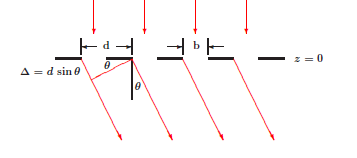
\includegraphics[scale=1.2]{Bilder/Gitterbeugung_Schema.PNG}
		\end{center}
		\caption[Gitterbeugung Schema]{Schematische Darstellung der Beugung an einem Gitter}
		\label{fig:Gitterbeugung_Schema}
	\end{figure}
	Abbildung \ref{fig:Gitterbeugung_Schema} zeigt schematisch die Entstehung des Beugungsbildes durch den Gangunterschied zwischen zwei benachbarten Strahlen am Gitter. Wenn dieser Gangunterschied ein ganzzahliges Vielfaches der Wellenlänge ist, liegt konstruktive Interferenz vor und es ist ein Maximum zu sehen. Dies führt auf die wichtige Bedingung
	\begin{equation}
	d \sin (\theta) = n \lambda.
	\label{eq:Maximumsbedingung}
	\end{equation}
	Dabei bezeichnet $n$ die Ordnung des Maximums. An dieser Beziehung lassen sich einige wichtige Bedingungen ablesen. Damit beobachtbare Beugung auftritt, muss $\lambda < d$ gelten. Die maximal beobachtbare Ordnung ist $n_{max} = \dfrac{d}{\lambda}$. \\
	Wenn die Gitterebene nicht exakt senkrecht zum einfallenden Strahl steht, muss ein Gangunterschied zwischen den Strahlen vor dem Gitter berücksichtigt werden. Wenn $\varphi$ der Winkel zwischen der Senkrechten zum Lichtstrahl und der Gitterebene und $\theta$ der Beobachtungswinkel ist, kann Gl. \ref{eq:Maximumsbedingung} verallgemeinert werden zu:
	\begin{equation}
	d(\sin(\varphi) + \sin(\theta - \varphi)) = n \lambda
	\label{eq:VerallgemeinerteMaximumsbedingung}
	\end{equation}
	
	\subsubsection{Auflösungsvermögen eines Gitters}
	Für die Trennung zweier nah beieinander liegender Spektrallinien $\lambda$ und $\lambda + \Delta \lambda$ müssen nach dem Rayleigh-Kriterium das erste Beugungsmaximum der ersten Linie mit dem ersten Beugungsminimum der zweiten Linie zusammenfallen. Aus dieser Bedingung lässt sich für das Auflösungsvermögen eines Gitters die Beziehung
	\begin{equation}
	A \equiv \dfrac{\lambda}{\Delta \lambda} = n \cdot N
	\label{eq:AuflösungsvermögenGitterspektrometer}
	\end{equation}
	herleiten. Dabei ist $n$ die Ordnung des betrachteten Maximums und $N$ die Zahl der beleuchteten Spalte des Gitters.
	
	\subsection{Aufbau und Durchführung}
	\begin{figure}
		\begin{center}
			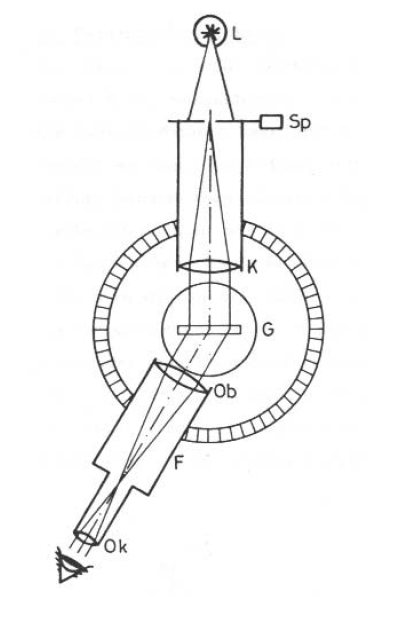
\includegraphics[scale=0.5]{Bilder/Schematischer_Aufbau_Gitterspektrometer.PNG}
		\end{center}
		\caption[Gitterspektrometer Aufbau Schema]{Schematische Darstellung des Versuchaufbaus der Beugung an einem Gitter}
		\label{fig:Versuchsaufbau_Gitterbeugung_Schema}
	\end{figure}
	Abbildung \ref{fig:Versuchsaufbau_Gitterbeugung_Schema} zeigt schematisch den Aufbau eines Gitterspektrometers.\\
	Eine Spektrallampe wird vor ein Kollimatorrohr gestellt. Dieses dient dazu, den Strahlengang möglichst parallel auf das Gitter zu schicken. An dem der Lampe zugewandten Ende des Kollimatorrohres ist ein in der Breite einstellbarer Spalt, der als zu beobachtender "Gegenstand" dient. Das Gitter steht auf einem Teller und wird dort (so gut wie möglich) senkrecht zum Kollimatorrohr aufgestellt. Sowohl das Gitter als auch das Kollimatorrohr werden einmal eingestellt und sollten danach nicht mehr bewegt werden. Bewegt wird nur das Fernrohr, mit dem die Beobachtung stattfindet. Dieses ist dazu auf einem drehbaren Arm angebracht, der mit einem Nonius verbunden ist, sodass ein Winkel abgelesen werden kann, mit dem dann die Beugung gemessen wird.\\
	Zunächst muss ein Fehler auf die Winkelmessung bestimmt werden. Dazu wird die nullte Ordnung zehnmal gemessen. Um wirklich zehn einzelne, voneinander unabhängige Messungen zu erhalten, wird das Maximum jedes Mal komplett neu angefahren. Bei den nachfolgenden Messungen wird angenommen, dass der Fehler auf die Winkelmessung immer gleich ist und der Fehler aus der Rauschmessung übernommen. Da hierfür die Nullte Ordnung verwendet wird, kann der Mittelwert der Rauschmessung als Nullniveau verwendet werden. Die gemessenen Winkel müssen also immer als Abweichung von diesem Nullniveau betrachtet werden.\\
	Für die Bestimmung der Gitterkonstanten eines (laut Herstellerangabe) sehr feinen Gitters muss eine Lampe mit vielen Spektrallinien im sichtbaren Bereich verwendet werden, da nach Gl. \ref{eq:Maximumsbedingung} nur wenige Ordnung beobachtbar sind. In diesem Fall wurde hierfür die Cadmium-Lampe verwendet. Es werden ausgewählte Spektrallinien in den beobachtbaren Ordnung angefahren und die Winkel gemessen. Wichtig ist, dass die Linien in Ordnung auf beiden Seiten der nullten Ordnung vermessen werden, um in der Anpassung berücksichtigen zu können, dass die Gitterebene nicht perfekt senkrecht zum einfallenden Strahl stand.\\
	Zur Bestimmung der Wellenlänge der Spektrallinien einer anderen Lampe wird muss die Lampe ausgewechselt werden. Da hier eine Quecksilber-Cadmium Lampe verwendet wurde, muss darauf geachtet werden, dass nur die Quecksilber-Linien sinnvoll vermessen werden können. Die Durchführung ist identisch zu der Durchführung der Messung der Gitterkonstanten.\\
	Zur Bestimmung des Auflösungsvermögens wird die Lampe durch eine andere ausgetauscht, die zwei nah beieinander liegende Spektrallinien hat. Hier wurden die beiden roten Linien der Natrium-Lampe verwendet. Es wird eine Leiste mit unterschiedlichen Blenden auf das Kollimatorrohr angebracht. Die Blenden haben Breiten in 0,5mm Schritten startend bei 0,5mm.\\
	Die rote Doppellinie wird in erster Ordnung angefahren und in dem Okular so gelegt, dass sie gut sichtbar nicht zu weit am Rand liegt. Es ist darauf zu achten, dass das Fadenkreuz am Okular nicht die beiden Linien trennt. Anschließend wird in der Leiste der Blenden nach und nach eine kleinere Blende eingestellt und immer wieder überprüft, ob die beiden Linien noch getrennt werden können oder nicht.
	
	\subsection{Bestimmung der Gitterkonstanten}
	
	\begin{table}
		\begin{center}
			\begin{tabular}{|c|}
				\hline
				Winkel \\
				\hline
				84$^{\circ}$ 35'\\
				\hline
				84$^{\circ}$ 32'\\
				\hline
				84$^{\circ}$ 32'\\
				\hline
				84$^{\circ}$ 31'\\
				\hline
				84$^{\circ}$ 32'\\
				\hline
				84$^{\circ}$ 32'\\
				\hline
				84$^{\circ}$ 33'\\
				\hline
				84$^{\circ}$ 33'\\
				\hline
				84$^{\circ}$ 33'\\
				\hline
				84$^{\circ}$ 32'\\
				\hline
			\end{tabular}
			\caption{Ergebnisse der Winkelmessung der nullten Ordnung.}
			\label{tab:RohdatenRauschmessungGitter}
		\end{center}
	\end{table}
	
	\begin{table}
		\begin{center}
			\begin{tabular}{|c|c|c|c|}
				\hline
				Ordnung & Wellenlänge [nm] & Messung 1 & Messung 2\\
				\hline
				2 & 643,85 & - & -\\
				\hline
				2 & 508,58 & 48$^{\circ}$ 21' & 47$^{\circ}$ 51'\\
				\hline
				2 & 479,99 & 50$^{\circ}$ 08' & 50$^{\circ}$ 09'\\
				\hline
				2 & 467,81 & 51$^{\circ}$ 06' & 51$^{\circ}$ 01'\\
				\hline
				1 & 643,85 & 62$^{\circ}$ 02' & 62$^{\circ}$ 04'\\
				\hline
				1 & 508,58 & 66$^{\circ}$ 51' & 66$^{\circ}$ 52'\\
				\hline
				1 & 479,99 & 67$^{\circ}$ 50' & 67$^{\circ}$ 53'\\
				\hline
				1 & 467,81 & 68$^{\circ}$ 20' & 68$^{\circ}$ 20'\\
				\hline
				-1 & 643,85 & 108$^{\circ}$ 05' & 101$^{\circ}$ 04'\\
				\hline
				-1 & 508,58 & 102$^{\circ}$ 51' & 102$^{\circ}$ 45'\\
				\hline
				-1 & 479,99 & 101$^{\circ}$ 41' & 101$^{\circ}$ 40'\\
				\hline
				-1 & 467,81 & 101$^{\circ}$ 15' & 101$^{\circ}$ 14'\\
				\hline
				-2 & 643,85 & - & -\\
				\hline
				-2 & 508,58 & 124$^{\circ}$ 24' & 124$^{\circ}$ 31'\\
				\hline
				-2 & 479,99 & 121$^{\circ}$ 39' & 121$^{\circ}$ 35'\\
				\hline
				-2 & 467,81 & 120$^{\circ}$ 30' & 120$^{\circ}$ 30'\\
				\hline
			\end{tabular}
			\caption{Ergebnisse der Winkelmessung der nullten Ordnung.}
			\label{tab:RohdatenBestimmungGitterkonstante}
		\end{center}
	\end{table}
	
	\begin{figure}
		\begin{center}
			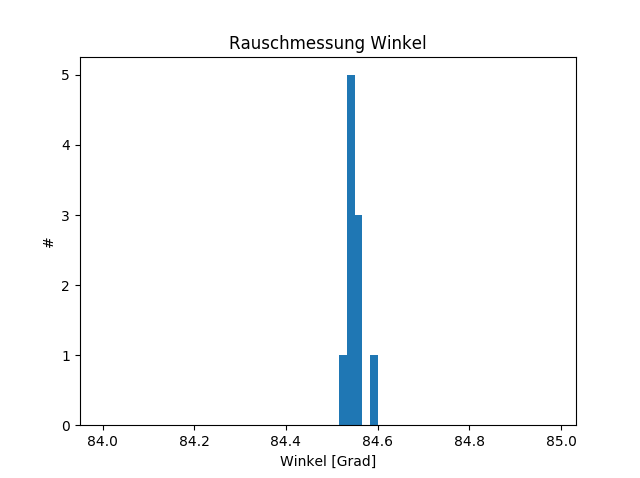
\includegraphics[scale=0.7]{Bilder/Rauschmessung_Winkelmessung_Nullte_Ordnung.png}
		\end{center}
		\caption[Rauschmessung Winkelmessung]{Verteilung der gemessenen Winkel der nullten Ordnung}
		\label{fig:Rauschmessung_Winkel_Gitter}
	\end{figure}
	
	\begin{figure}
		\begin{center}
			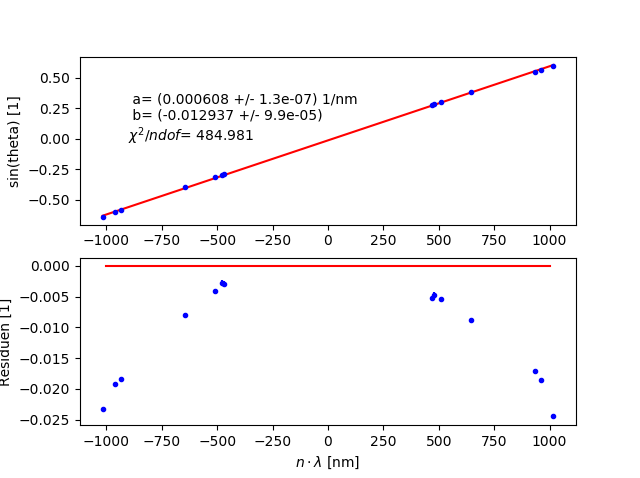
\includegraphics[scale=0.9]{Bilder/First_Fit_Gitterkonstante.png}
		\end{center}
		\caption[Erster Fit Gitterkonstante]{Erster Geradenfit zur Bestimmung der Gitterkonstante}
		\label{fig:FirstFit_Gitterkonstante}
	\end{figure}
	
	\begin{figure}
		\begin{center}
			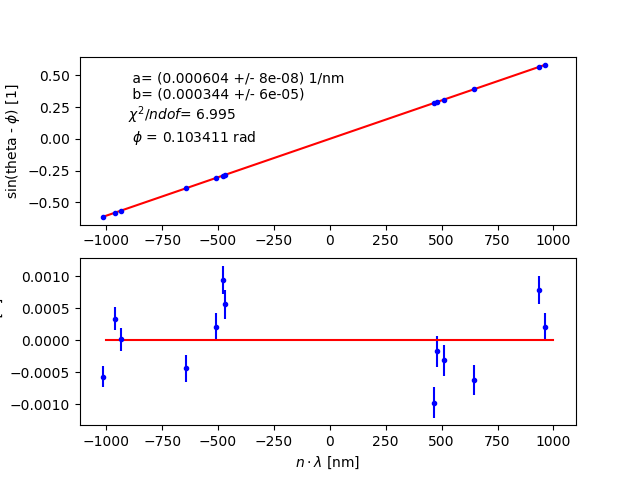
\includegraphics[scale=0.9]{Bilder/Anpassung_Gitterkonstante.png}
		\end{center}
		\caption[Fit Gitterkonstante]{Geradenfit mit minimalem $\chi ^2$ zur Bestimmung der Gitterkonstante}
		\label{fig:Fit_Gitterkonstante}
	\end{figure}
	
	Die gemessenen Winkel der nullten Ordnung sind in Tabelle \ref{tab:RohdatenRauschmessungGitter} aufgeführt. Aus den Winkel lassen sich Mittelwert und Fehler bestimmen zu:
	\begin{equation*}
	\bar{\alpha} = 84^{\circ} \quad 32,5' \qquad und \qquad \sigma_{\alpha} = 1,02'
	\end{equation*}
	Das Histogramm in Abbildung \ref{fig:Rauschmessung_Winkel_Gitter} zeigt, dass die gemessenen Winkel der nullten Ordnung einer Gaußverteilung folgen.
	
	Die gemessenen Winkel $\beta$ für die gegebenen Wellenlängen der Cadmium-Lampe sind in Tabelle \ref{tab:RohdatenBestimmungGitterkonstante} aufgeführt.\\
	Der Beobachtungswinkel $\theta$ berechnet sich nun zu 
	\begin{equation}
	\theta = \bar{\alpha} - \bar{\beta}.
	\end{equation}
	Damit und mit der Annahme, dass die Fehler auf die Winkelmessungen immer gleich sind berechnet sich der Fehler auf den Beobachtungswinkel als
	\begin{equation}
	\sigma _{\theta} = \sigma _{\alpha} + \sigma _{\beta} = 2 \cdot \sigma _{\alpha}
	\end{equation}
	
	Trägt man den Sinus des Winkels gegen das Produkt aus Wellenlänge und Ordnung auf, würde man gemäß Gl. \ref{eq:Maximumsbedingung} eine Gerade mit Steigung $\dfrac{1}{d}$ erwarten. Ein Geradenfit an die entstehende Gerade ist in Abbildung \ref{fig:FirstFit_Gitterkonstante} gezeigt. In den Residuen ist eine sehr deutliche Systematik zu sehen. Dies deutet darauf hin, dass das verwendete Modell nicht stimmt, der Winkel $\varphi$ zwischen der Senkrechten zum einfallenden Lichtstrahl und der Gitterebene nicht null ist. Daher muss eine Anpassung der Form von Gl. \ref{eq:VerallgemeinerteMaximumsbedingung} gemacht werden. Dazu wurde die Gleichung umgestellt zu
	\begin{equation}
	\sin (\theta - \varphi) = \dfrac{n \cdot \lambda}{d} - \sin (\varphi).
	\end{equation}
	In dieser Gleichung ist nur $\theta$ fehlerbehaftet, daher muss auch nur in der Y-Koordinate ein Fehler berechnet werden. Dieser berechnet sich aus gauß'scher Fehlerfortpflanzung zu:
	\begin{equation}
	\sigma _Y = \sigma _{\theta} \cdot \cos(\theta - \varphi) = 2 \cdot \sigma _{\alpha} \cdot \cos(\theta - \varphi)
	\end{equation}
	Nun kann (bei festem $\varphi$) eine lineare Regression in $\theta$ durchgeführt werden. Die sich bei unterschiedlichen $\varphi$ ergebenden $\chi ^2$ können nun für $\varphi$ minimiert werden. Damit ergibt sich für die Anpassung mit minimalem $\chi ^2$ der Fit, der in Abbildung \ref{fig:Fit_Gitterkonstante} gezeigt wird. Dabei ergibt sich der Winkel, um den das Gitter aus der idealen Position verdreht ist zu:
	\begin{equation*}
	\varphi = 0,107658 \, rad = 6 ^{\circ} \; 10,1'
	\end{equation*}
	Dann kann aus der Steigung $a$ der Geraden die Gitterkonstante berechnet werden zu:
	\begin{equation}
	d = \dfrac{1}{a}
	\end{equation}
	Beim Invertieren bleibt der relative Fehler gleich, daher errechnet sich der Fehler auf die Gitterkonstante zu:
	\begin{equation}
	\dfrac{\sigma_d}{d} = \dfrac{\sigma_a}{a} \quad \Leftrightarrow \quad \sigma_d = \sigma_a \cdot \dfrac{d}{a}
	\end{equation}
	Damit ergeben sich die Gitterkonstante und der statistische Fehler auf diese zu:
	\begin{equation*}
	d = (1658,91 \pm 0,34)nm
	\end{equation*}
Die Herstellerangabe für das Gitter war $600 \dfrac{Spalte}{mm}$. Umgerechnet ergibt sich damit die Herstellerangabe für die Gitterkonstante zu:
\begin{equation*}
d_{Hersteller} = \dfrac{1}{600} \dfrac{mm}{Strich} = 1666,\bar{6} nm
\end{equation*}
Das Messergebnis liegt damit knapp 23$\sigma$ neben der Herstellerangabe. Diese Abweichung ist nicht verwunderlich, da der relative Fehler auf die gemessene Gitterkonstante mit ca. 0,205 \textperthousand $\;$ sehr klein ist.
	
	\subsection{Bestimmung der Wellenlänge}
	
	Die gemessenen Winkel der Spektrallinien sind in Tabelle \ref{tab:rohdaten_wellenlängen} dargestellt. Als statistischer Fehler auf die Einzelmessung wird weiterhin $\sigma_{einzel} = \SI{0.000295}{rad}$ angenommen (siehe Bestimmung Gitterkonstante). Da alle Winkel doppelt gemessen wurden ergibt sich für die Winkel relativ zur Nullten Ordnung
	\begin{equation}
	\theta_{gesucht} = \theta_{Nullte\;Ordnung} - \theta_{Andere\;Ordnung}
	\end{equation}
	und damit
	\begin{equation}
	\sigma_{stat} = \frac{\sqrt{2}}{\sqrt{2}} \sigma_{einzel} = \sigma_{einzel}.
	\end{equation}
	\begin{table}
		\centering
		\begin{tabular}{|c|c|c|}
			\hline
			Ordnung & Winkel Messung 1 & Winkel Messung 2 \\
			\hline
			\hline
			0 & \SI{84}{\degree} \SI{35}{\arcminute} &  \SI{84}{\degree} \SI{53}{\arcminute} \\
			\hline
			&&\\
			Linie 1&& \\
			\hline
			1 & \SI{70}{\degree} \SI{29}{\arcminute} & \SI{70}{\degree} \SI{29}{\arcminute} \\
			\hline
			-1 & \SI{98}{\degree} \SI{51}{\arcminute} & \SI{98}{\degree} \SI{41}{\arcminute} \\
			\hline
			
			&&\\
			Linie 2&& \\
			\hline
			1 & \SI{69}{\degree} \SI{20}{\arcminute} & \SI{69}{\degree} \SI{21}{\arcminute} \\
			\hline
			2 & \SI{53}{\degree} \SI{00}{\arcminute} & \SI{53}{\degree} \SI{00}{\arcminute} \\
			\hline
			-1 & \SI{99}{\degree} \SI{52}{\arcminute} & \SI{99}{\degree} \SI{51}{\arcminute} \\
			\hline
			-2 & \SI{116}{\degree} \SI{35}{\arcminute} & \SI{116}{\degree} \SI{31}{\arcminute} \\
			\hline
			
			&&\\
			Linie 3&&\\
			\hline
			1 & \SI{65}{\degree} \SI{22}{\arcminute} & \SI{65}{\degree} \SI{22}{\arcminute} \\
			\hline
			2 & \SI{43}{\degree} \SI{41}{\arcminute} & \SI{43}{\degree} \SI{36}{\arcminute} \\
			\hline
			-1 & \SI{103}{\degree} \SI{55}{\arcminute} & \SI{103}{\degree} \SI{51}{\arcminute} \\
			\hline
			-2 & \SI{126}{\degree} \SI{10}{\arcminute} & \SI{126}{\degree} \SI{10}{\arcminute} \\
			\hline
			
			&&\\
			Linie 4&&\\
			\hline
			1 & \SI{64}{\degree} \SI{14}{\arcminute} & \SI{64}{\degree} \SI{15}{\arcminute} \\
			\hline
			2 & \SI{40}{\degree} \SI{47}{\arcminute} & \SI{40}{\degree} \SI{46}{\arcminute} \\
			\hline
			-1 & \SI{105}{\degree} \SI{03}{\arcminute} & \SI{105}{\degree} \SI{00}{\arcminute} \\
			\hline
			-2 & \SI{129}{\degree} \SI{07}{\arcminute} & \SI{129}{\degree} \SI{08}{\arcminute} \\
			\hline
			
			&&\\
			Linie 5&&\\
			\hline
			1 & \SI{64}{\degree} \SI{10}{\arcminute} & \SI{64}{\degree} \SI{09}{\arcminute} \\
			\hline
			2 & \SI{40}{\degree} \SI{37}{\arcminute} & \SI{40}{\degree} \SI{35}{\arcminute} \\
			\hline
			-1 & \SI{105}{\degree} \SI{10}{\arcminute} & \SI{105}{\degree} \SI{05}{\arcminute} \\
			\hline
			-2 & \SI{129}{\degree} \SI{21}{\arcminute} & \SI{129}{\degree} \SI{23}{\arcminute} \\
			\hline
			
			
		\end{tabular}
		\caption{Gemessene Winkel der fünf zu bestimmenden Spektrallinien.}
		\label{tab:rohdaten_wellenlängen}
	\end{table}
	Es gilt:
	\begin{equation}
	d \sin \theta = n \lambda.
	\end{equation}
	
	Damit erhält man die Wellenlänge $\lambda$ als Steigung einer angepassten Geraden an die Messwerte mit $n$ auf der x- und $d \sin \theta$ auf der y-Achse. Diese
	
	Für den systematischen Fehler aus der Messung der Gitterkonstante gilt jeweils:
	
	\begin{equation}
	\sigma_{syst} = \frac{\sin \theta}{n} \sigma_d
	\end{equation}
	
	Um die Auswirkung dieses Fehlers auf das Ergebnis abzuschätzen, wurde die Verschiebemethode verwendet. Dazu werden die Messpunkte mit ihren statistischen Fehlern um die systematischen Fehler verschoben, einmal nach oben und einmal nach unten,   \\
	
	\begin{equation}
	d \sin(\theta)_{i, -} = d \sin(\theta) - \sigma _{syst}
	\end{equation}
	bzw.
	\begin{equation}
	d \sin(\theta)_{i, +} = d \sin(\theta) + \sigma _{syst}
	\end{equation}
	
	und man wiederholt jeweils die lineare Regression. So erhält man zwei neue Werte $\lambda_{-}$ bzw. $\lambda_{+}$ für die Wellenlänge. Der systematische Fehler auf die Wellenlänge ist dann der Mittelwert der Abweichungen:
	\begin{equation}
	\Delta \lambda _{syst} = ( |\lambda_{-}-\lambda| + |\lambda_{+} - \lambda|)/2 .
	\end{equation}
	
	Ein beispielhafter Fit ist in Abbildung \ref{fig:fit_wellenlaengen} anhand Linie 4 dargestellt, dabei wurde darauf verzichtet den systematischen Fehler darzustellen, da er noch kleiner ist als der statistische Fehler.
	
	\begin{figure}
		\centering
		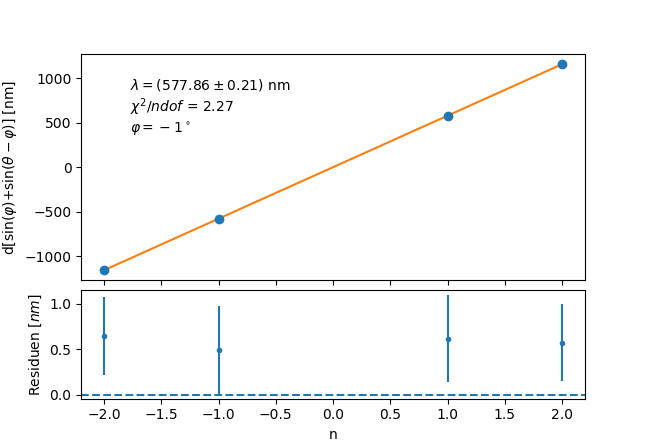
\includegraphics[scale=1.0]{Bilder/Gitter_Regression_Wellenlaengen_Linie_4.png}
		\caption{Dargestellt sind die gemessenen Winkel einer Spektrallinie gegen die Ordnung mit linearem Fit. Daraus ergibt sich die Wellenlänge der Linie mit statistischem Fehler.}
		\label{fig:fit_wellenlaengen}
	\end{figure}
	
	Die Ergebnisse mit statistischem sowie systematischen Fehler sind in Tabelle \ref{tab:ergebnisse_wellenlängen} zusammengefasst.
	
	\begin{table}
		\centering
		\begin{tabular}{|c|c|c|c|}
			\hline
			Linie & Wellenlänge $\pm$ stat $\pm$ sys [nm] & Literaturwert [nm] & Abweichung\\
			\hline
			\hline
			1 & 405.32 $\pm$ 2.15 $\pm$ 0.08 & 404.66 & +0.3$\sigma$ \\
			\hline
			2 & 436.74 $\pm$ 0.86 $\pm$ 0.09 & 435.83 & +1.6$\sigma$ \\
			\hline
			3 & 547.06 $\pm$ 1.06 $\pm$ 0.11 & 546.07 & +0.9$\sigma$ \\
			\hline
			4 & 578.01 $\pm$ 1.17 $\pm$ 0.12 & 576.96 & +0.9$\sigma$ \\
			\hline
			5 & 580.24 $\pm$ 1.29 $\pm$ 0.12 & 579.07 & +0.9$\sigma$\\
			\hline
		\end{tabular}
		\caption{Berechnete Wellenlängen der betrachteten Spektrallinien}
		\label{tab:ergebnisse_wellenlängen}
	\end{table}
	
	Unsere Messwerte stimmen im Rahmen ihrer Fehler mit den Literaturwerten überein.
	
	\subsection{Bestimmung der Auflösung}
	
	Die verwendete Natrium D Doppellinie mit einem Abstand von \SI{0.59}{nm} erfordert ein Auflösungsvermögen von A = $\frac{\lambda}{\Delta\lambda} \approx 1000 $, um beide Linien voneinander trennen zu können.
	
	Die die Breite der vorgeschalteten Blende ergibt zusammen mit der Gitterkonstanten ein Auflösungsvermögen, diese sind in Tabelle \ref{tab:gitter_auflösung} zusammengefasst. Dabei haben wir die Doppellinie in erster Ordnung beobachtet.
	
	Im Experiment konnten wir bei Verwendeng der \SI{2.5}{mm} breiten Blende gut erkennen, dass es sich um zwei Linien handelt. Die \SI{2.0}{mm} breite Blende machte es bereits kaum erkennbar und mit der \SI{1.5}{mm} Blende war die Doppellinie für uns nicht mehr als solche zu erkennen.
	
	Diese Ergebnisse entsprechen der Erwartung.
	
	\begin{table}
		\centering
		\begin{tabular}{|c|c|}
			\hline
			Blende [mm] & Auflösungsvermögen \\
			\hline \hline
			2.5 & 1507 \\
			\hline
			2.0 & 1206 \\
			\hline
			1.5 & 904 \\
			\hline
		\end{tabular}
		\caption{Auflösungsvermögen des Gitters in erster Ordnung mit vorgeschalteter Blende.}
		\label{tab:gitter_auflösung}
	\end{table}
	
\subsection{Zusammenfassung}
Die Rauschmessung für die Winkelbestimmung ergab einen Fehler in der erwarteten Größenordnung einer Bogenminute.\\
Das Gitter wurde beim Versuchsaufbau offenbar nicht senkrecht zum einfallenden Strahl gestellt. Hier gab es eine Abweichung von 6$^{\circ}$. Dieser Fehler kann allerdings rausgerechnet werden, daher hat dies keinen Einfluss auf das Endergebnis.\\
Die Gitterkonstante konnte mit einem relativen Fehler von gerade einmal 0,205 \textperthousand $\;$ bestimmt werden, obwohl das $\chi ^2$ pro Freiheitsgrad mit ca. 6 nicht so schlecht ist. Die Abweichung von der Herstellerangabe liegt bei ca. 4,654 \textperthousand $\;$. Dies entspricht ca. 23 Standardabweichungen. Die Gitterkonstante konnte also mit geringer relativer Abweichung von der Herstellerangabe und sehr sehr kleinem Fehler bestimmt werden.
	
	
\end{document}
